\let\negmedspace\undefined
\let\negthickspace\undefined
\documentclass[journal]{IEEEtran}
\usepackage[a5paper, margin=10mm, onecolumn]{geometry}
%\usepackage{lmodern} % Uncomment if needed for pdflatex
\usepackage{tfrupee} % Include tfrupee package

\setlength{\headheight}{1cm} % Set the height of the header box
\setlength{\headsep}{0mm}     % Set the distance between the header box and the top of the text

\usepackage{gvv-book}
\usepackage{gvv}
\usepackage{cite}
\usepackage{amsmath,amssymb,amsfonts,amsthm}
\usepackage{algorithmic}
\usepackage{graphicx}
\usepackage{textcomp}
\usepackage{xcolor}
\usepackage{txfonts}
\usepackage{listings}
\usepackage{enumitem}
\usepackage{mathtools}
\usepackage{gensymb}
\usepackage{comment}
\usepackage[breaklinks=true]{hyperref}
\usepackage{tkz-euclide} 
\usepackage{listings}
%\usepackage{gvv}                                        
\def\inputGnumericTable{}                                 
\usepackage[latin1]{inputenc}                                
\usepackage{color}                                            
\usepackage{array}                                            
\usepackage{longtable}                                       
\usepackage{calc}                                             
\usepackage{multirow}                                         
\usepackage{hhline}                                           
\usepackage{ifthen}                                           
\usepackage{lscape}
\usepackage{tikz}
\usepackage{circuitikz}
\usepackage{standalone} % For including external TikZ files

\begin{document}

\bibliographystyle{IEEEtran}
\vspace{3cm}

\title{10.4.1.2.4}
\author{EE24BTECH11066 - YERRA AKHILESH}
% \maketitle
% \newpage
% \bigskip
{\let\newpage\relax\maketitle}

\renewcommand{\thefigure}{\theenumi}
\renewcommand{\thetable}{\theenumi}
\setlength{\intextsep}{10pt} % Space between text and floats

\numberwithin{equation}{enumi}
\numberwithin{figure}{enumi}
\renewcommand{\thetable}{\theenumi}
\textbf{Question}:\\

On comparing the ratio's $\frac{a_1}{a_2}, \frac{b_1}{b_2} \text{ and } \frac{c_1}{c_2}$, find out whether the following pair of linear equations are consistent, or inconsistent.\\
$$2x - 3y = 8 $$
$$4x - 6y = 9$$

\textbf{Solution : }\\

For the first equation:
\begin{align}
    a_1 = 2,\\ b_1 = -3,\\ c_1 = 8
\end{align}
and For the second equation:
\begin{align}
    a_2 = 4,\\ b_2 = -6,\\ c_2 = 9
\end{align}
Compare the ratio's,
\begin{align}
    \frac{a_1}{a_2} = \frac{2}{4} = \frac{1}{2}\\
    \frac{b_1}{b_2} = \frac{-3}{-6} = \frac{1}{2}\\
    \frac{c_1}{c_2} = \frac{8}{9}
\end{align}
from the above results
\begin{align}
    \frac{a_1}{a_2} =\frac{b_1}{b_2} \neq \frac{c_1}{c_2}
\end{align}
We know that if:
\begin{align}
    \frac{a_1}{a_2} =\frac{b_1}{b_2} \neq \frac{c_1}{c_2}
\end{align}
then the equations are \textbf{inconsistent}, meaning they represent parallel lines with \textbf{no solution}

We aim to solve the system of equations using LU decomposition:
\begin{align}
    2x - 3y &= 8, \\
    4x - 6y &= 9.
\end{align}

\section*{Step 1: Represent the system in matrix form}
\begin{align}
    A &= \begin{bmatrix} 2 & -3 \\ 4 & -6 \end{bmatrix}, \quad
    \vec{x} = \begin{bmatrix} x \\ y \end{bmatrix}, \quad
    \vec{b} = \begin{bmatrix} 8 \\ 9 \end{bmatrix}.
\end{align}
Thus, the system becomes:
\begin{align}
    A \vec{x} &= \vec{b}.
\end{align}

\section*{Step 2: Decompose \(A\) into \(L\) and \(U\)}
To find \(L\) (lower triangular matrix) and \(U\) (upper triangular matrix), we perform Gaussian elimination.

\subsection*{Row Reduction}
Start with:
\begin{align}
    A = \begin{bmatrix} 2 & -3 \\ 4 & -6 \end{bmatrix}.
\end{align}
Perform the row operation \(R_2 \to R_2 - 2R_1\):
\begin{align}
    \begin{bmatrix} 2 & -3 \\ 4 & -6 \end{bmatrix}
    \xrightarrow{R_2 \to R_2 - 2R_1}
    \begin{bmatrix} 2 & -3 \\ 0 & 0 \end{bmatrix}.
\end{align}
The second row becomes zero, indicating that the matrix \(A\) is singular $\brak{\text{det }A = 0}$.

\subsection*{Define \(L\) and \(U\)}
From the row reduction, we can write:
\begin{align}
    L &= \begin{bmatrix} 1 & 0 \\ 2 & 1 \end{bmatrix}, \quad
    U = \begin{bmatrix} 2 & -3 \\ 0 & 0 \end{bmatrix}.
\end{align}
Thus:
\begin{align}
    A = L \cdot U.
\end{align}

\section*{Step 3: Solve the system using forward and back substitution}

\subsection*{Forward Substitution: Solve \(L \vec{y} = \vec{b}\)}
\begin{align}
    \begin{bmatrix} 1 & 0 \\ 2 & 1 \end{bmatrix}
    \begin{bmatrix} y_1 \\ y_2 \end{bmatrix} &=
    \begin{bmatrix} 8 \\ 9 \end{bmatrix}.
\end{align}
From the first row:
\begin{align}
    y_1 &= 8.
\end{align}
From the second row:
\begin{align}
    2y_1 + y_2 &= 9, \quad \text{which gives } y_2 = -7.
\end{align}
Thus:
\begin{align}
    \vec{y} = \begin{bmatrix} 8 \\ -7 \end{bmatrix}.
\end{align}

\subsection*{Back Substitution: Solve \(U \vec{x} = \vec{y}\)}
\begin{align}
    \begin{bmatrix} 2 & -3 \\ 0 & 0 \end{bmatrix}
    \begin{bmatrix} x \\ y \end{bmatrix} &=
    \begin{bmatrix} 8 \\ -7 \end{bmatrix}.
\end{align}
From the second row:
\begin{align}
    0x + 0y &= -7 \quad \text{(contradiction!)}.
\end{align}

\section*{Conclusion}
The LU decomposition process reveals that the system is \textbf{inconsistent}. The matrix \(A\) is singular (its determinant is zero), and the system does not have a solution. The inconsistency arises because the equations contradict each other.
\begin{figure}[!ht]
		\centering
		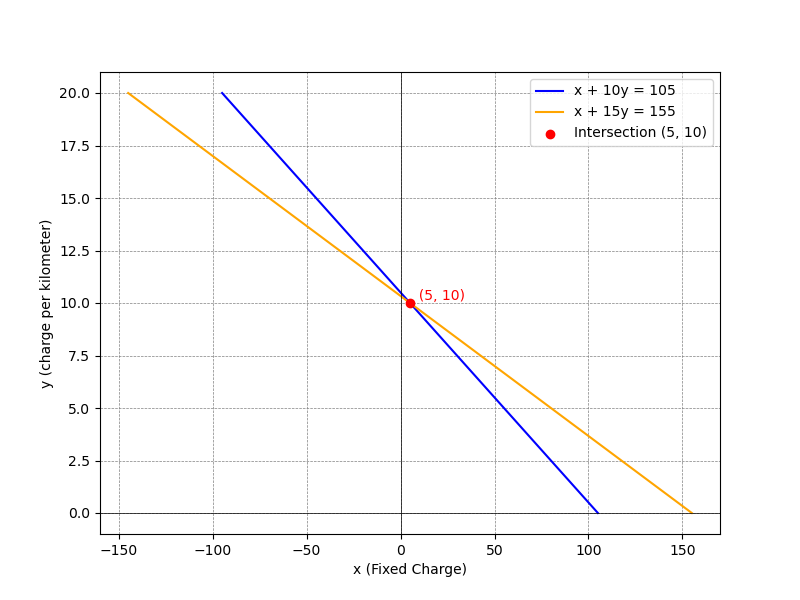
\includegraphics[width=\columnwidth]{figs/Figure_1.png}
		\caption{Solution of the system of linear equations}
		\label{stemplot}
	\end{figure}
\end{document}
